\documentclass[10pt]{article}

%%%%%%%%%%%%%%%%%%%%%%%%%%%%%%%%%%%%%%%%%%%%%%%%%%%%%%%%%%%%%%%%%%%%%%%%%%%%%%%%
% LaTeX Imports
%%%%%%%%%%%%%%%%%%%%%%%%%%%%%%%%%%%%%%%%%%%%%%%%%%%%%%%%%%%%%%%%%%%%%%%%%%%%%%%%
\usepackage{amsfonts}                                                   % Math fonts
\usepackage{amsmath}                                                    % Math formatting
\usepackage{amssymb}                                                    % Math formatting
\usepackage{amsthm}                                                     % Math Theorems
\usepackage{arydshln}                                                   % Dashed hlines
\usepackage{attachfile}                                                 % AttachFiles
\usepackage{cancel}                                                     % Cancelled math
\usepackage{caption}                                                    % Figure captioning
\usepackage{color}                                                      % Nice Colors
\input{./lib/dragon.inp}                                                % Tikz dragon curve
\usepackage[ampersand]{easylist}                                        % Easy lists
\usepackage{fancyhdr}                                                   % Fancy Header
\usepackage[T1]{fontenc}                                                % Specific font-encoding
%\usepackage[margin=1in, marginparwidth=2cm, marginparsep=2cm]{geometry} % Margins
\usepackage{graphicx}                                                   % Include images
\usepackage{hyperref}                                                   % Referencing
\usepackage[none]{hyphenat}                                             % Don't allow hyphenation
\usepackage{lipsum}                                                     % Lorem Ipsum Dummy Text
\usepackage{listings}                                                   % Code display
\usepackage{marginnote}                                                 % Notes in the margin
\usepackage{microtype}                                                  % Niceness
\usepackage{lib/minted}                                                 % Code display
\usepackage{multirow}                                                   % Multirow tables
\usepackage{pdfpages}                                                   % Include pdfs
\usepackage{pgfplots}                                                   % Create Pictures
\usepackage{rotating}                                                   % Figure rotation
\usepackage{setspace}                                                   % Allow double spacing
\usepackage{subcaption}                                                 % Figure captioning
\usepackage{tikz}                                                       % Create Pictures
\usepackage{tocloft}                                                    % List of Equations
%%%%%%%%%%%%%%%%%%%%%%%%%%%%%%%%%%%%%%%%%%%%%%%%%%%%%%%%%%%%%%%%%%%%%%%%%%%%%%%%
% Package Setup
%%%%%%%%%%%%%%%%%%%%%%%%%%%%%%%%%%%%%%%%%%%%%%%%%%%%%%%%%%%%%%%%%%%%%%%%%%%%%%%%
\hypersetup{%                                                           % Setup linking
    colorlinks=true,
    linkcolor=black,
    citecolor=black,
    filecolor=black,
    urlcolor=black,
}
\RequirePackage[l2tabu, orthodox]{nag}                                  % Nag about bad syntax
\renewcommand*\thesection{\arabic{section} }                             % Reset numbering
\renewcommand{\theFancyVerbLine}{ {\arabic{FancyVerbLine} } }              % Needed for code display
\renewcommand{\footrulewidth}{0.4pt}                                    % Footer hline
\setcounter{secnumdepth}{3}                                             % Include subsubsections in numbering
\setcounter{tocdepth}{3}                                                % Include subsubsections in toc
%%%%%%%%%%%%%%%%%%%%%%%%%%%%%%%%%%%%%%%%%%%%%%%%%%%%%%%%%%%%%%%%%%%%%%%%%%%%%%%%
% Custom commands
%%%%%%%%%%%%%%%%%%%%%%%%%%%%%%%%%%%%%%%%%%%%%%%%%%%%%%%%%%%%%%%%%%%%%%%%%%%%%%%%
\newcommand{\nvec}[1]{\left\langle #1 \right\rangle}                    %  Easy to use vector
\newcommand{\ma}[0]{\mathbf{A} }                                         %  Easy to use vector
\newcommand{\mb}[0]{\mathbf{B} }                                         %  Easy to use vector
\newcommand{\abs}[1]{\left\lvert #1 \right\rvert}                       %  Easy to use abs
\newcommand{\pren}[1]{\left( #1 \right)}                                %  Big parens
\let\oldvec\vec
\renewcommand{\vec}[1]{\oldvec{\mathbf{#1} } }                            %  Vector Styling
\newtheorem{thm}{Theorem}                                               %  Define the theorem name
\newtheorem{definition}{Definition}                                     %  Define the definition name
\definecolor{bg}{rgb}{0.95,0.95,0.95}
\newcommand{\java}[4]{\vspace{10pt}\inputminted[firstline=#2,
                                 lastline=#3,
                                 firstnumber=#2,
                                 gobble=#4,
                                 frame=single,
                                 label=#1,
                                 bgcolor=bg,
                                 linenos]{java}{#1} }
\newcommand{\python}[4]{\vspace{10pt}\inputminted[firstline=#2,
                                 lastline=#3,
                                 firstnumber=#2,
                                 gobble=#4,
                                 frame=single,
                                 label=#1,
                                 bgcolor=bg,
                                 linenos]{python}{#1} }
\newcommand{\js}[4]{\vspace{10pt}\inputminted[firstline=#2,
                                 lastline=#3,
                                 firstnumber=#2,
                                 gobble=#4,
                                 frame=single,
                                 label=#1,
                                 bgcolor=bg,
                                 linenos]{js}{#1} }
%%%%%%%%%%%%%%%%%%%%%%%%%%%%%%%%%%%%%%%%%%%%%%%%%%%%%%%%%%%%%%%%%%%%%%%%%%%%%%%%
% Beginning of document items - headers, title, toc, etc...
%%%%%%%%%%%%%%%%%%%%%%%%%%%%%%%%%%%%%%%%%%%%%%%%%%%%%%%%%%%%%%%%%%%%%%%%%%%%%%%%
\pagestyle{fancy}                                                       %  Establishes that the headers will be defined
\fancyhead[LE,LO]{Computer Systems Notes}                                  %  Adds header to left
\fancyhead[RE,RO]{Zoe Farmer}                                       %  Adds header to right
\cfoot{ \thepage }
\lfoot{CSCI 2400}
\rfoot{Han}
\title{Computer Systems Notes}
\author{Zoe Farmer}

%%%%%%%%%%%%%%%%%%%%%%%%%%%%%%%%%%%%%%%%%%%%%%%%%%%%%%%%%%%%%%%%%%%%%%%%%%%%%%%%
% Beginning of document items - headers, title, toc, etc...
%%%%%%%%%%%%%%%%%%%%%%%%%%%%%%%%%%%%%%%%%%%%%%%%%%%%%%%%%%%%%%%%%%%%%%%%%%%%%%%%
\pagestyle{fancy}                                                       %  Establishes that the headers will be defined
\fancyhead[LE,LO]{Homework 8}                                  %  Adds header to left
\fancyhead[RE,RO]{Zoe Farmer}                                       %  Adds header to right
\cfoot{\mlptikz[size=0.25in, text=on, textposx=0, textposy=0, textvalue=\thepage, textscale=0.75in]{applejack}}
\lfoot{APPM 3570}
\rfoot{Kleiber}
\title{Homework 8}
\date{Kleiber}
\author{Zoe Farmer - 101446930}
%%%%%%%%%%%%%%%%%%%%%%%%%%%%%%%%%%%%%%%%%%%%%%%%%%%%%%%%%%%%%%%%%%%%%%%%%%%%%%%%
% Beginning of document items - headers, title, toc, etc...
%%%%%%%%%%%%%%%%%%%%%%%%%%%%%%%%%%%%%%%%%%%%%%%%%%%%%%%%%%%%%%%%%%%%%%%%%%%%%%%%
\begin{document}

\maketitle

\begin{table}[!ht]
    \centering
    \scalebox{1.5}{%
    \begin{tabular}{|l|l|l|l||l|}
        \hline
        1 & 2 & 3 & 4 & T\\
        \hline
        & & & &\\
        \hline
    \end{tabular}
    }
\end{table}

\begin{easylist}[enumerate]
    \ListProperties(Hide1=50, Space1=1cm)
    @ \textit{Chapter 5 \#7 --} The density function of $X$ is given by

    \[
        f(x) =
        \begin{cases}
            a + b x^2 &\to 0 \le x \le 1\\
            0 &\to Otherwise
        \end{cases}
    \]

    If $E(X) = \frac{3}{5}$, find $a$ and $b$.
    @@ We can rewrite $E(X)$ as the below and solve for $a$ and $b$.

    \[
        \begin{aligned}
            E(X) &=& \int^1_0 x \left( a + b x^2 \right) \, dx\\
                 &=& \int^1_0 ax + b x^3  \, dx\\
                 &=& \left. \frac{ax^2}{2} + \frac{bx^4}{4} \right|^1_0\\
                 &=& \frac{a}{2} + \frac{b}{4} = \frac{3}{5}\\
                 &=& \frac{2a + b}{4} = \frac{3}{5}\\
                 &=& 10a + 5b = 12\\
             10a &=& 12 - 5b \Rightarrow a = \frac{12 - 5b}{10}\\
             1 &=& \int^1_0 \frac{12 - 5b}{10} + bx^2 \, dx\\
             && \boxed{b = \frac{6}{5} \qquad a = \frac{3}{5}}
        \end{aligned}
    \]

    @ \textit{Chapter 5 \# 10 --} Trains headed for destination $A$ arrive at the train station at 15-minute intervals
    starting at 7 AM, whereas trains headed for destination $B$ arrive at 15-minute intervals starting at 7:05 AM.
    @@ If a certain passenger arrives at the station at a time uniformly distributed between 7 and 8 AM and then gets on
    the first train that arrives, what proportion of time does he or she go to destination $A$?
    @@@ We can use the definition of a uniform distribution and find that the probability that a passenger arrives at
    any given time is 1/60. Train $A$ arrives at $\{0700, 0715, 0730, 0745, 0800\}$ while train $B$ arrives at
    $\{0705,0720,0735,0750\}$. The probability that the passenger gets on any one train can be expressed as

    \[
        \begin{aligned}
            A \to &\{ \frac{1}{60},\frac{1}{60},\frac{1}{60},\frac{1}{60},\frac{1}{60} \}\\
            B \to &\{ \frac{1}{60},\frac{1}{60},\frac{1}{60},\frac{1}{60} \}
        \end{aligned}
    \]

    Now to find the total probability of either destination, we can simply sum the sets and obtain the probability that
    he boards train $A$ to be $\frac{1}{12}$ and the probability that he boards train $B$ to be $\frac{1}{15}$. He will
    board train $A$ more often.

    @@ What if the passenger arrives at a time uniformly distributed between 7:10 and 8:10 AM?
    @@@ Now our sets adjust slightly.

    \[
        \begin{aligned}
            A \to &\{ 0700, 0715, 0730, 0745, 0800 \}\\
            B \to &\{ 0705, 0720, 0735, 0750, 0805 \}\\
            \text{Rewriting with probabilities}\\
            A \to &\{ \frac{1}{60},\frac{1}{60},\frac{1}{60},\frac{1}{60},\frac{1}{60} \}\\
            B \to &\{ \frac{1}{60},\frac{1}{60},\frac{1}{60},\frac{1}{60},\frac{1}{60} \}\\
        \end{aligned}
    \]

    And we see that the probabilities are the same, $\frac{1}{12}$.

    @ \textit{Chapter 5 \# 11 --} A point is chosen at random on a line segment of length $L$. Interpret this statement,
    and find the probability that the ratio of the shorter to the longer segment is less than $\frac{1}{4}$.
    @@ If the probability that any point is chosen is equal, than we have a uniform distribution, and the probability
    that any given point being chosen is $\frac{1}{L}$. Let $X$ the ratio of the shorter to longer segments. We're
    interested in $P(X < 0.25) = 1 - P(X \ge 0.25)$.\newline

    Let's first find the probability that any given point is chosen.
    \[
        p(k; L) =
        \begin{cases}
            \frac{1}{L} &\to 0 \le k \le L\\
            0 &\to Otherwise
        \end{cases}
    \]

    Now let's look at the probability that the ratio is equal to any given number.

    \[
        f(k; L) =
        \begin{cases}
            p(k \cdot L; L) &\to k \ge 0\\
            0 &\to Otherwise
        \end{cases}
    \]

    Finally we can determine

    \[
        1 - P(X \ge 0.25) = 1 - \int_{0.25}^L \frac{1}{L} \, dx = \boxed{1 - \frac{1}{L} \cdot (L - 0.25)}
    \]

    @ \textit{Chapter 5 \# 13 --} You arrive at a bus stop at 10 o'clock, knowing that the bus will arrive at some time
    uniformly distributed between 10 and 10:30.
    @@ What is the probability that you will have to wait longer than 10 minutes?
    @@@ If the arrival time is uniformly distributed, than we can assume that the mean time is 10:15, and that we can
    use the definition of the pdf of a uniform distribution, which states that a distribution is uniform if the pdf is
    equal to

    \[
        f(k; A, B) =
        \begin{cases}
            \frac{1}{B-A} &\to A \le k \le B\\
            0 &\to Otherwise
        \end{cases} =
        \begin{cases}
            \frac{1}{30} &\to 0 \le k \le 30\\
            0 &\to Otherwise
        \end{cases}
    \]

    Using this allows us to determine the cdf

    \[
        F(k; A, B) =
        \begin{cases}
            0 &\to x < A\\
            \frac{x-A}{B-A} &\to A \le k < B\\
            1 &\to x \ge B
        \end{cases} =
        \begin{cases}
            0 &\to x < 0\\
            \frac{x}{30} &\to 0 \le k < 30\\
            1 &\to x \ge 30
        \end{cases}
    \]

    By which we can determine $P(X > 10) = 1 - P(X \le 10) = 1 - \frac{1}{3} = \boxed{0.66667}$ where $X$ is the number
    of minutes needed to wait.

    @@ If, at 10:15, the bus has not yet arrived, what is the probability that you will have to wait at least an
    additional 10 minutes?
    @@@ We've now changed the time period, and thusly we need to adjust the probability distributions.

    \[
        F(k; A, B) =
        \begin{cases}
            0 &\to x < 0\\
            \frac{x}{15} &\to 0 \le k < 15\\
            1 &\to x \ge 15
        \end{cases}
    \]

    By which we can new determine $P(X \ge 10) = \frac{2}{3} = \boxed{0.66667}$.

    @ \textit{Chapter 5 \# 16 --} The annual rainfall (in inches) in a certain region is normally distributed with $\mu
    = 40$ and $\sigma = 4$. What is the probability that, starting with this year, it will take over 10 years before a
    year occurs having a rainfall of over 50 inches? What assumptions are you making?
    @@ Recall that a normally distributed random variable has the form

    \[
        f(x, \mu=40, \sigma=4) = \frac{1}{\sigma\sqrt{2\pi}} e^{-\frac{(x-\mu)^2}{2\sigma^2} } =
        \frac{1}{4\sqrt{2\pi}} e^{-\frac{(x-40)^2}{32}}
    \]

    If we let $X$ be how many inches of rain the region receives, we are then interested in $P(X > 50) = 1 - P(X \le
    50)$, which we can write as such.

    \[ 1 - \int^{50}_0 \frac{1}{4\sqrt{2\pi}} e^{-\frac{(x-40)^2}{32}} \, dx = 0.00620967 \]

    This number is the probability that any given year has more than 50 inches of rain. If we now let $Y$ be the random
    variable denoting how many years it is until 50 inches is received, then we can create a new Geometric distribution
    with the probability of success being our previously calculated probability.

    \[ f(k; p=0.00620967) = {(1 - p)}^{k-1} p = {(1 - 0.00620967)}^{k-1} 0.00620967 \]

    We now find $P(Y > 10) = 1 - P(Y \le 10)$ to be $\boxed{0.933775}$. This is with the assumption that each year's
    rainfall is independent of the previous years.

    @ \textit{Chapter 5 \# 18 --} Suppose that $X$ is a normal random variable with mean 5. If $P\{X > 9\} = 0.2$,
    approximately what is $Var(X)$?
    @@ We can rewrite the given probability to that in terms of a cdf.

    \[
        \begin{aligned}
            P(X > 9) = 1 - P(X \le 9) =
            1 - \int^9_{-\infty} \frac{1}{\sigma\sqrt{2\pi}} e^{-\frac{(x-5)^2}{2\sigma^2} } \, dx &=& 0.2\\
            \int^9_{-\infty} \frac{1}{\sigma\sqrt{2\pi}} e^{-\frac{(x-5)^2}{2\sigma^2} } \, dx &=& 0.8\\
            \sigma &=& \boxed{4.75273}
        \end{aligned}
    \]

    @ \textit{Chapter 5 \# 23 --} One thousand independent rolls of a fair die will be made. Compute an approximation to
    the probability that the number 6 will appear between 150 and 200 times inclusively. If the number 6 appears exactly
    200 times, find the probability that the number 5 will appear less than 150 times.
    @@ We can model this as a binomial distribution, where the probability of success is 1/6 and the number of ``flips''
    is 1000.

    \begin{figure}[!ht]
        \centering
        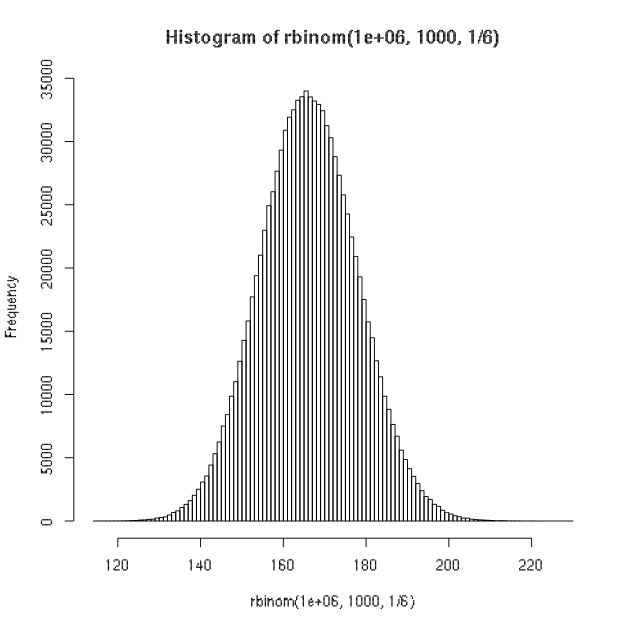
\includegraphics[scale=0.5]{./img/binomial0.png}
    \end{figure}

    Which can be rewritten and solved for the appearance of the number 6 between 150 and 200 times.

    \[ \sum^{200}_{k=150} \binom{1000}{k} {(1/6)}^k {1 - (1/6)}^{1000 - k} \, dk \approx 0.9264531 \]

    If the number 6 appears \textit{exactly} 200 times than we can rewrite the problem to examine 5 instead.

    \[ \sum^{149}_{k=0} \binom{800}{k} {(1/5)}^k {1 - (1/5)}^{800 - k} \, dk \approx 0.17698455 \]

    @ \textit{Chapter 5 \# 26 --} Two types of coins are produced at a factory: a fair coin and a biased one that comes
    up heads 55 percent of the time. We have one of these coins, but do not know whether it is a fair coin or a biased
    one. In order to ascertain which type of coin we have, we shall perform the following statistical test: We shall
    toss the coin 1000 times. If the coin lands on heads 525 or more times, then we shall conclude that it is a biased
    coin, whereas if it lands on heads less than 525 times, then we shall conclude that it is a fair coin. If the coin
    is actually fair, what is the probability that we shall reach a false conclusion?  What would it be if the coin were
    biased?
    @@ We can model this as a binomial distribution:

    \begin{figure}[!ht]
        \centering
        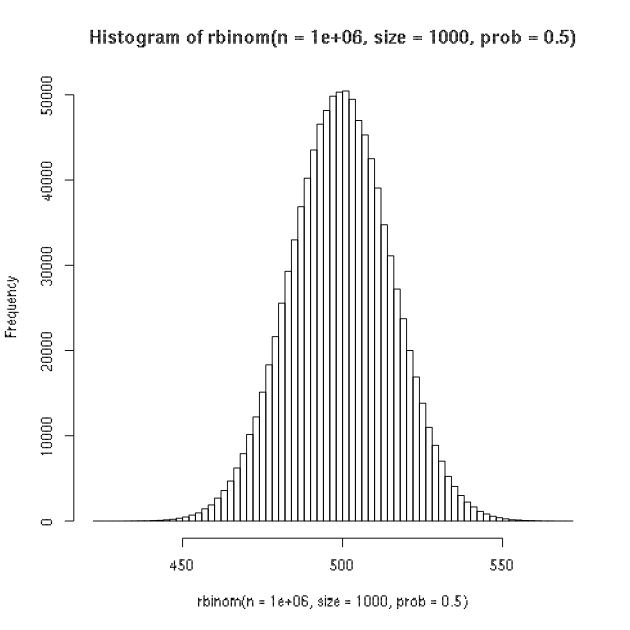
\includegraphics[scale=0.5]{./img/binomial.png}
    \end{figure}

    Whereupon we see that not only is the binomial distribution uniform, it also tells us the probability that a coin
    will yield 525 or more heads as

    \[ \sum^\infty_{k=525} \binom{1000}{k} 0.5^k {0.5}^{1000 - k} \, dk = 0.0606071 \]

    This number is the probability that any given coin will have 525 or more heads. This means that if we are given a
    fair coin, $\approx 5\%$ of the time we will incorrectly categorize the coin. On the flipside, if our coin is biased
    our probability shifts from 0.5 to 0.55, and our equation becomes

    \[ \sum^\infty_{k=525} \binom{1000}{k} 0.55^k {0.55}^{1000 - k} \, dk = 0.9473182 \]

    And we see that we catch biased coins 95\% of the time.

    @ \textit{Chapter 5 \# 27 --} In 10,000 independent tosses of a coin, the coin landed on heads 5800 times. Is it
    reasonable to assume that the coin is not fair? Explain.
    @@ In this situation, if someone was bored enough to flip a coin 10,000 times which resulted in 58\% heads, it would
    be a reasonable assumption to assume that the coin is not fair. Sure, there is a margin of error in this assumption
    due to the fact that the coin is supposed to be entirely random, and thereby you cannot be 100\% sure that it is an
    unfair coin, however this is enough trial to see a consistent trend.

    @ \textit{Chapter 5 \# 7 --} The standard deviation of $X$, denoted $SD(X)$, is given by

    \[
        SD(X) = \sqrt{Var(X)}
    \]

    Find $SD(aX + b)$ if $X$ has variance $\sigma^2$.
    @@ We can simply use the definition of standard deviation. The standard deviation of $aX + b$ is simply $a \cdot
    \sigma$ where $\sigma$ is the standard deviation of $X$, defined as the square root of the variance.

    @ \textit{Chapter 5 \# 9 --} Show that $Z$ is a standard normal random variable, then, for $x > 0$,
    @@ $P(Z > x) = P(Z < -x)$
    @@@ The definition we need here is that of the cdf of a continuous variable, which is defined as

    \[
        F(x) = \int^x_{-\infty} f(y) \, dy
    \]

    Using this we can rewrite this as the below equation and solve.

    \[
        \begin{aligned}
        1 - \int^x_{-\infty} f(y) \, dy &=& 1 - \int^\infty_{-x} f(y) \, dy\\
        \int^x_{-\infty} f(y) \, dy &=& \int^\infty_{-x} f(y) \, dy\\
        \end{aligned}
    \]

    Since we are working with a uniform distribution, then these two parts are equal.

    @@ $P(|Z| > x) = 2P(Z > x)$
    @@@ Using our definitions from before it is trivial to see that since we have a uniform distribution, everything on
    the left side of the mean is a mirror of the right side of the mean. This means that if we look at the absolute
    value of $Z$, we are in fact looking at the two equal end parts, which is equal to twice one.
    @@ $P(|Z| < x) = 2P(Z < x) - 1$
    @@@ Again, we can use our previous definitions to prove this. Similar to (b) we see that the absolute value
    indicates a doubled probability, however in this case we are concerned about the space contained, because it is much
    larger, therefore we need to pull out the middle part, which has probability 1.

    @ \textit{Chapter 5 \# 10 --} Let $f(x)$ denote the probability density function of a normal random variable with
    mean $\mu$ and variance $\sigma^2$. Show that $\mu - \sigma$ and $\mu + \sigma$ are points of inflection of this
    function. That is, show that $f(x) = 0$ when $x = \mu - \sigma$ or $x = \mu + \sigma$.
    @@ A normal distribution has form

    \[ f(x, \mu, \sigma) = \frac{1}{\sigma\sqrt{2\pi}} e^{ -\frac{(x-\mu)^2}{2\sigma^2} } \]

    With first derivative

    \[ \frac{df(x, \mu, \sigma)}{dx} = -\frac{e^{-\frac{{(x - \mu)}^2}{2 \sigma^2}} (x - \mu)}{\sqrt{2 \pi} \sigma^3} \]

    And second derivative

    \[ \frac{d}{dx} = \frac{(x-\mu )^2 e^{-\frac{(x-\mu )^2}{2 \sigma ^2}}}{\sqrt{2 \pi } \sigma ^5}-
                        \frac{e^{-\frac{(x-\mu )^2}{2 \sigma^2}}}{\sqrt{2 \pi } \sigma ^3} \]

    Now if we simply plug in $\mu \pm \sigma$ we can see that the second derivative is equal to zero, which by
    definition makes these two points inflection points.
\end{easylist}

\end{document}
